	% !TeX spellcheck = en_GB
	\begin{figure}[!htb]
	  \setlength{\unitlength}{\textwidth}
	
	        \begin{picture}(1,0.8)(-0.02,0)
	
	 
	      \put(0.08,0.4){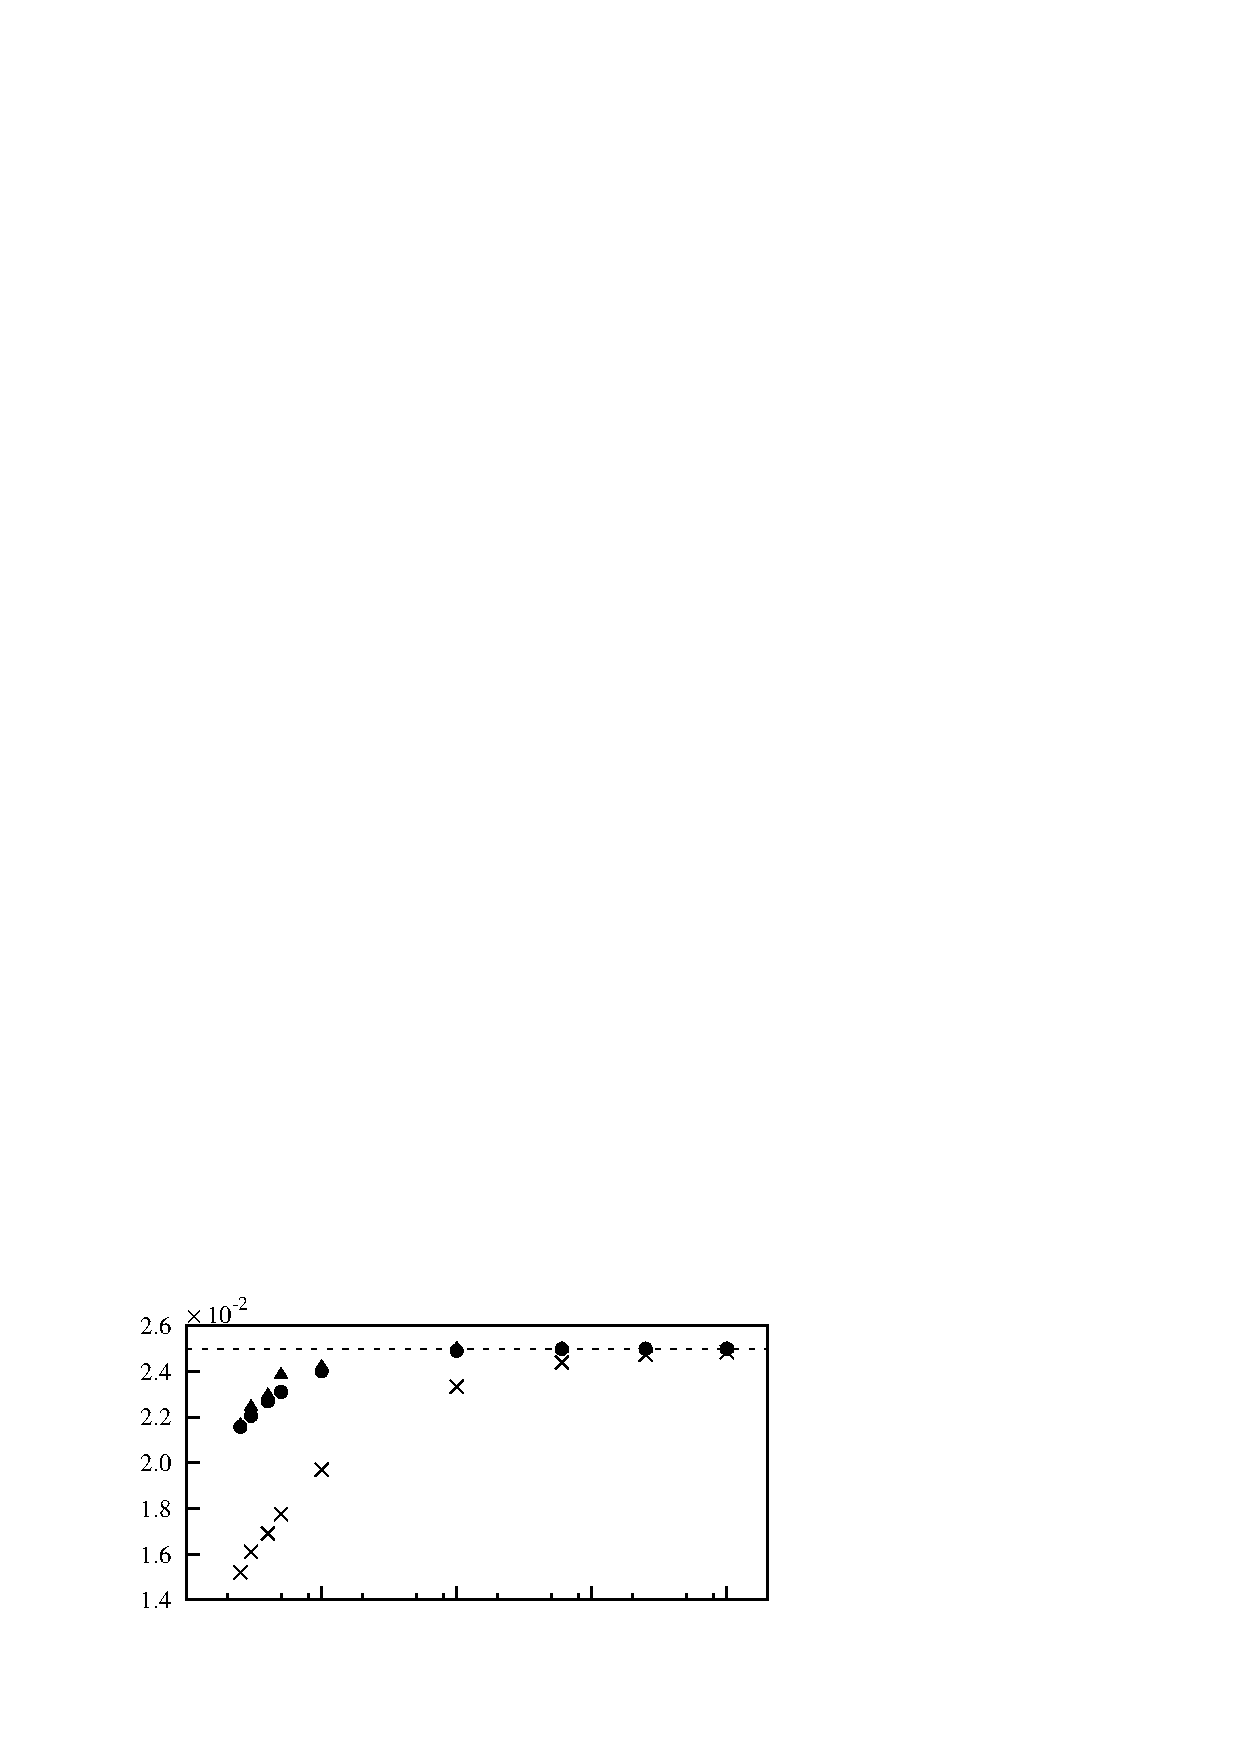
\includegraphics[width=0.75\unitlength]{{./chapter-frequnecy-response/fnp/freq015}.eps}}
	      \put(0.04,0.02){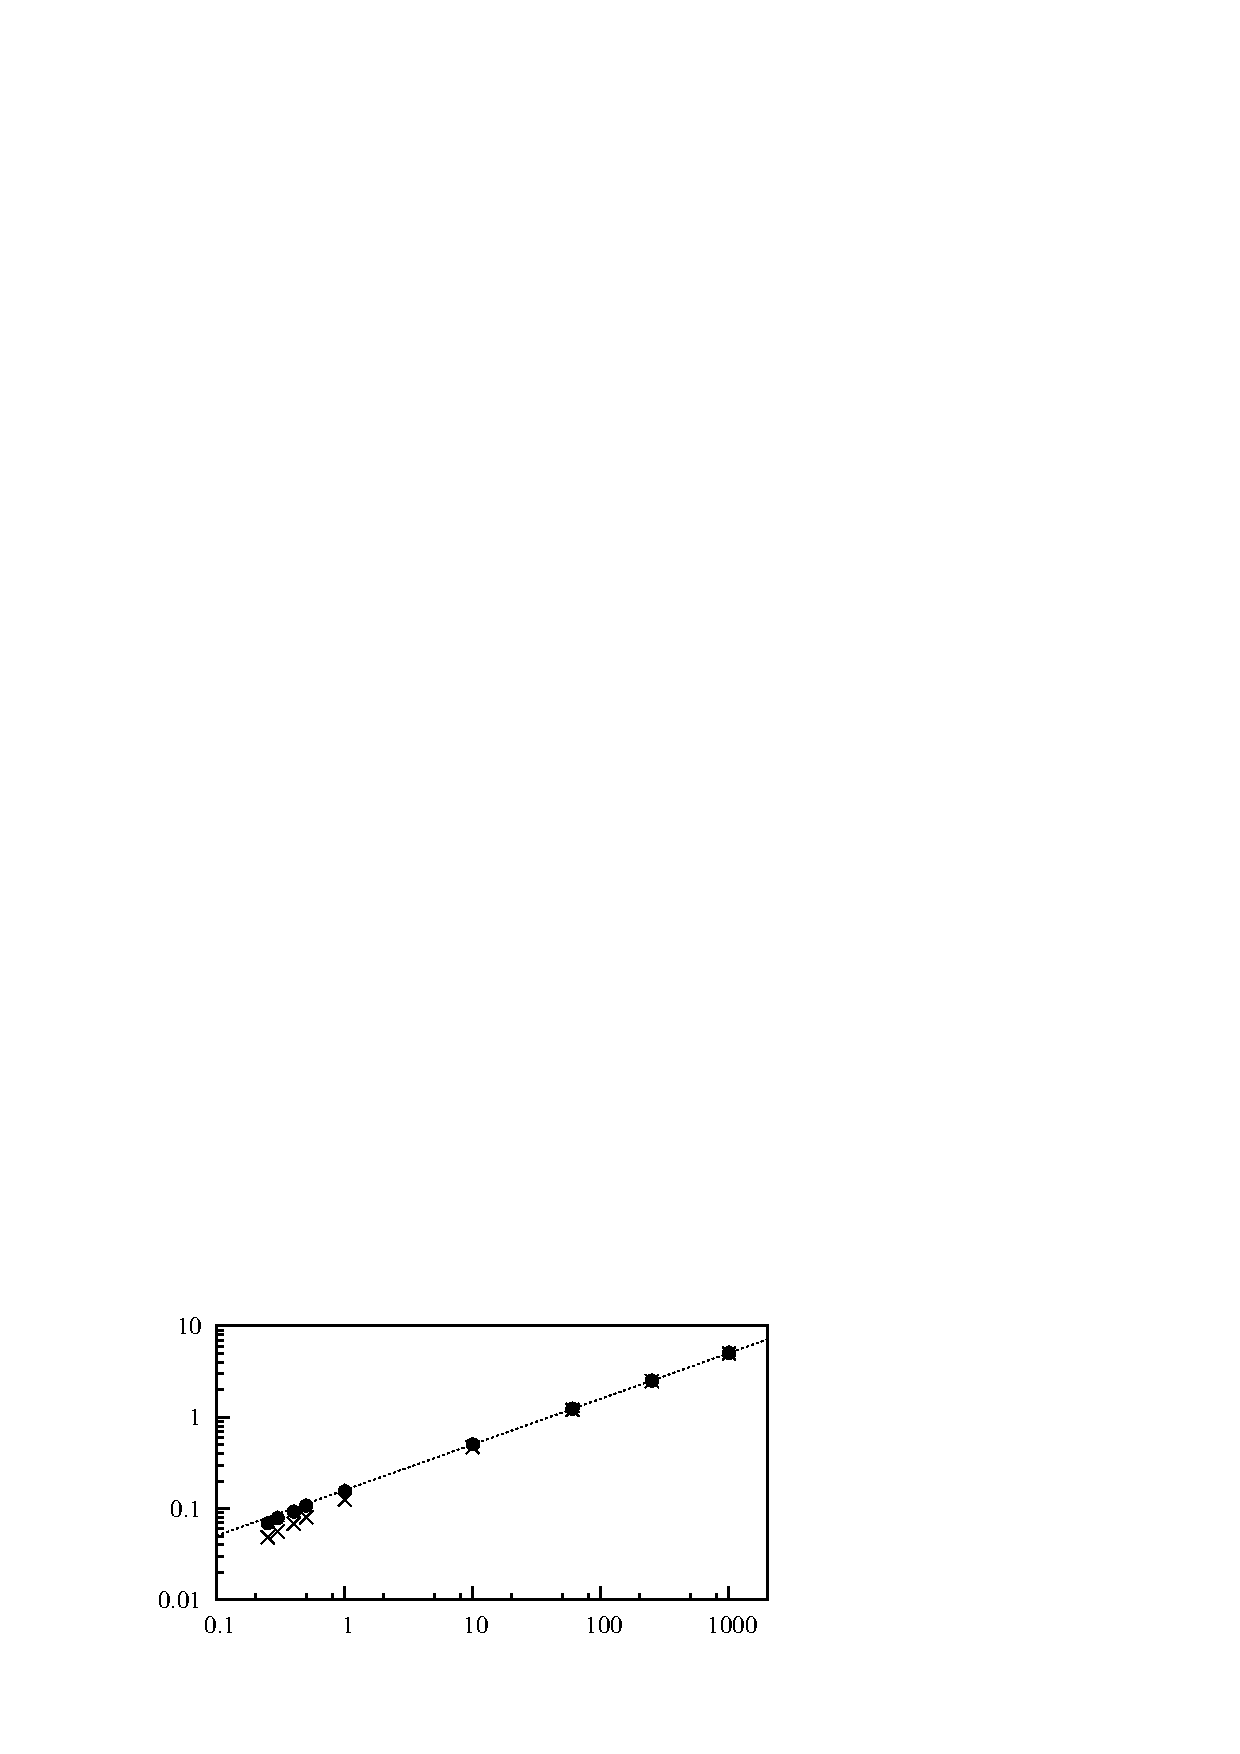
\includegraphics[width=0.8\unitlength]{{./chapter-frequnecy-response/fnp/freq015_2}.eps}}
	
	      \put(0.47,0.00){\massstiff}
	      
	      
	     
	       \put(0.06,0.235){$\displaystyle\frac{f_{i}D m^{*}}{U}$}
	        \put(0.058,0.58){$\displaystyle\frac{f_{i}D }{U}$}
	      
	
	      \put(0.17,0.47){\small(a)}
	      \put(0.17,0.085){\small(b)}
	      
	    \end{picture}
	
	  \caption{Frequency data as a function of \massstiff, (a) without and (b) with scaling with \mstar. Frequency obtained using QSS simulations, DNS simulations and the linear frequency equation (Eq:\ref{eqn:linear_freq_final}). $f_{i}$ is the type of frequency i.e. \freqdns,\freqqss ,\freqlin. Data present $f_{lin}$ ($\bullet$), $f_{QSS}$ (\ding{115}) and $f_{DNS}$ ($\times$) at $\massdamp=0.15$, $\reynoldsnumber=200$ and undamped natural frequency, $f=0.025$ (\dashedrule). }
	    \label{fig:pi2-015-freq}
	\end{figure}
	
	 %vspace{10cm}
